\documentclass[12pt,pdf,notheorems]{beamer}
\usetheme{Warsaw}
\usepackage[T2A]{fontenc}
\usepackage[utf8]{inputenc}
\usepackage[english,russian]{babel}
\usepackage{amsfonts, amssymb, amsmath, amsthm}
\usepackage{graphicx}
\usepackage{subcaption}

\graphicspath{{./resources/presentation/}}

%\input {m:/papers/symb.tex}
%\input {../def.tex}
\renewcommand{\leq}{\leqslant}
\renewcommand{\geq}{\geqslant}
\renewcommand{\phi}{\varphi}
\newcommand{\R}{\mathbb{R}}
\newcommand{\E}{\mathbf{E}}
\renewcommand{\C}{\mathcal{C}}
\newcommand{\bF}{\bar{\mathcal{F}}}
\newcommand{\F}{\mathcal{F}}
\newcommand{\cY}{\check{Y}}
\newcommand{\wY}{\widetilde{Y}}
\newcommand{\wDelta}{\widetilde{\Delta}}
\renewcommand{\wp}{\widetilde{p}}
\newcommand{\wq}{\widetilde{q}}
\newcommand{\wf}{\widetilde{f}}
\newcommand{\wrho}{\widetilde{\rho}}
\newcommand{\hq}{\widehat{q}}
\newcommand{\eps}{\varepsilon}

\newtheorem{theorem}{Теорема}
%\newtheorem{lemma}{Лемма}
%\newtheorem{remark}{Замечание}

\title{Обучение без учителя. Разделение смеси распределений. Кластеризация.}
\author{Федяев~И. \and Понизова~В.}
\date[2019] % (optional)

\begin{document}
\frame{\titlepage}

\section[Обучение без учителя]{Обучение без учителя}

\begin{frame}
	Обучение без учителя (Unsupervised learning) --- раздел машинного обучения, в котором изучается класс задач обработки данных, в которых известны
	только описания множества объектов (признаки объектов) из обучающей выборки, и требуется обнаружить внутренние зависимости, существующие
	между объектами.
\end{frame}

\begin{frame}
	Типы задач обучения без учителя:
	\begin{itemize}
		\item Кластеризация
		\item Поиск ассоциативных правил
		\item Заполнение пропущенных значений
		\item Сокращение размерности
		\item Визуализация данных
	\end{itemize}
\end{frame}

\section[Кластеризация]{Кластеризация}
\subsection[Постановка задачи]{Постановка задачи}

\begin{frame}
Пусть имеется подмножество $X \subset \R^n$, которое мы будем называть пространством объектов.

	Некоторый конечный набор $X^m = \{x_1, \dots, x_m\}$ --- обучающая выборка.

	$\rho: X \times X \rightarrow [0, \infty)$ --- функция расстояния между объектами.

Необходимо найти множество кластеров $Y$ и алгоритм кластеризации $a: X \rightarrow Y$ такие, что:
	\begin{itemize}
		\item каждый кластер состоит из близких объектов (относительно $\rho$);
		\item объекты разных кластеров различались существенно.
	\end{itemize}
\end{frame}

\begin{frame}\frametitle{Некорректность}
Решение задачи кластеризации принципиально неоднозначно:
	\begin{itemize}
		\item точной постановки задачи кластеризации нет;
		\item существует много критериев качества кластеризации;
		\item существует много эвристических методов кластеризации;
		\item число кластеров, как правило, не известно заранее;
		\item результат кластеризации сильно зависит от метрики $\rho$, выбор которой также не однозначен.
	\end{itemize}
\end{frame}

\begin{frame}\frametitle{Цели кластеризации}
	\begin{itemize}
		\item Упростить дальнейшую обработку данных
		\item Сократить объём хранимых данных
		\item Поиск выбросов
		\item Построить иерархию множества объектов
	\end{itemize}
\end{frame}

\begin{frame}\frametitle{Алгоритмы кластеризации}
	\begin{itemize}
		\item Статистические методы (model-based)
			\begin{itemize}
				\item EM-алгоритм
				\item k-means
			\end{itemize}
		\item Эвристические методы
			\begin{itemize}
				\item Иерархическая агломеративная кластеризация
				\item FOREL
				\item DBSCAN
			\end{itemize}
	\end{itemize}
\end{frame}

\section[Статистические алгоритмы кластеризации]{Статистические алгоритмы кластеризации}
\subsection[Разделение смеси распределений. EM-алгоритм]{Разделение смеси распределений. EM-алгоритм}

\begin{frame}
	\frametitle{Смесь распределений}
	\textbf{Гипотеза:} выборка $X^m$ --- случайна, независима и взята из смеси распределений, плотность которой $p(x) = \sum_{j=1}^k w_j p_j(x;\theta_j), \sum_{j=1}^k w_j = 1$. 
\medskip

	$p_j(x;\theta_j)$ -- плотность распределения $j$-го кластера с параметрами $\theta_j$, 
	$w_j$ --- априорная вероятность кластера $j$.
\end{frame}

	\begin{frame}
	Предлагается, зная число кластеров $k$ и вид плотностей $p_j$, оценить параметры $w_j$ и $\theta_j$, 
	максимизируя логарифм функции правдоподобия 
		$$\ln \mathcal{L}(\{x_i\}; \{w_j\}; \{\theta_j\}) = \sum_{i=1}^m \ln \sum_{j=1}^k w_j p_j(x_i; \theta_j) \rightarrow \max_{\{w_j\}, \{\theta_j\}}$$ 
	при условии $\sum_{j=1}^k w_j =1; w_j \geq 0$.
\end{frame}

\begin{frame}
	\frametitle{Шаг E (expectation)} Пусть $p(x, \theta_j)$ --- плотность вероятности того, что объект $x$ получен из $j$-ой компоненты смеси.
	По формуле условной вероятности: $$p(x, \theta_j) = p(x) P(\theta_j~|~x) = w_j p_j(x; \theta_j).$$ Обозначим $g_{ij}= P(\theta_j~|~x)$. 
	По формуле Байеса:
	$$g_{ij} = \frac{w_j p_j(x_i; \theta_j)}{\sum_{s=1}^k w_{s} p_{s}(x_i; \theta_s) }.$$
\end{frame}

\begin{frame}
	\frametitle{Шаг M (maximization)} Максимизируем $$\ln \mathcal{L}(\{x_i\}; \{w_j\}; \{\theta_j\}) = \sum_{i=1}^m \ln \sum_{j=1}^k w_j p_j(x_i; \theta_j) \rightarrow \max_{\{w_j\}, \{\theta_j\}}$$
	при условии $\sum_{j=1}^k w_j =1$.
	Лагранжиан:
	$$L(\{w_j\}, \{ \theta_j\} ; \{x_i\}) = \sum_{i=1}^m \ln \sum_{j=1}^k w_j p_j(x_i; \theta_j) - \lambda \left( \sum_{j=1}^k w_j - 1 \right).$$
\end{frame}

\begin{frame}
	Из равенства нулю производной по $w_j$ следует $$w_j = \frac{1}{m} \sum_{i=1}^m g_{ij}, \quad j=1, \dots, k.$$

	Из равенства нулю производной по $\theta_j$ следует $$\theta_j = \arg \max_\theta \sum_{i=1}^m g_{ij} \ln p(x_i; \theta), \quad j=1, \dots, k.$$
\end{frame}

\begin{frame}\frametitle{Случай нормальных плотностей}
Пусть компоненты смеси имеют нормальные многомерные распределения со средними $\mu_j$ и матрицами ковариаций $\Sigma_j$, тогда 
имеем следующие оценки параметров
	$$\mu_j = \frac{1}{mw_j} \sum_{i=1}^m g_{ij} x_i,$$
	$$\Sigma_j = \frac{1}{mw_j} \sum_{i=1}^m g_{ij} (x_i - \mu_j) (x_i - \mu_j)^{\mathrm{T}}.$$
\end{frame}

\begin{frame}\frametitle{EM-алгоритм}
	\begin{enumerate}
		\item Вычислить начальное приближение $w_y, \theta_y$
		\item \textbf{Повторять}
		\item \quad E-шаг: $g_{ij}^0 = g_{ij}; \quad g_{ij} = \frac{w_j p_j(x_i; \theta_j)}{\sum_{s=1}^k w_{s} p_{s}(x_i; \theta_s) }$.
		\item \quad M-шаг:~$\theta_j = \arg \max_\theta \sum_{i=1}^m g_{ij} \ln p(x_i; \theta);$
		
			\quad  $w_j = \frac{1}{m} \sum_{i=1}^m g_{ij}$.
		\item \textbf{Пока} $\max_{i,j} |g_{ij} - g_{ij}^0| > \delta$.
	\end{enumerate}
\end{frame}

\begin{frame}
	\begin{figure}
		\centering
		\begin{subfigure}{0.4\linewidth}
			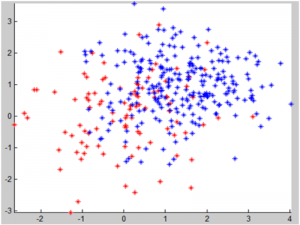
\includegraphics[scale=0.4]{EMTrue.png}
			\caption{Реальные данные}
		\end{subfigure}
		\begin{subfigure}{0.5\linewidth}
			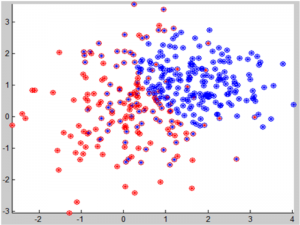
\includegraphics[scale=0.4]{EMModel.png}
			\caption{Результат кластеризации}
		\end{subfigure}
			\caption{Работа EM-алгоритма}
	\end{figure}
\end{frame}

\begin{frame}\frametitle{Плюсы и минусы}
	Достоинства:
	\begin{itemize}
	\item Для этого алгоритма есть более-менее чётко поставленная задача;
	\item Нет необходимости масштабировать признаки.
	\end{itemize}
	
	Недостатки
	\begin{itemize}
	\item Алгоритм неустойчив по начальным данным (то есть тем, которые инициализируют вектора параметров $w$ и $\theta$ на первой итерации);
	\item не позволяет определять количество k компонент смеси. Эта величина является структурным параметром алгоритма.
	\end{itemize}
\end{frame}

\subsection[k-means]{k-means}
\begin{frame}\frametitle{Алгоритм k-means}
	\begin{enumerate}
	\item Сформировать начальное приближение центров кластеров;
	\item \textbf{Повторять}
	\item \quad  Отнести каждый объект к ближайшему 

		\quad центру (аналог E-шага);
	\item \quad  Усреднить объекты в кластерах и получаем 

	        \quad новое положение центров (аналог M-шага);
	\item \textbf{Пока} состав кластеров не перестанет изменяться.
	\end{enumerate}
\end{frame}

\begin{frame}
	Алгоритм k-means можно получить из EM-алгоритма, если
	\begin{itemize}
		\item заменить подсчёт вероятностей $g_{ij}$ принадлежности $i$-го объекта $j$-ому кластеру на жёсткое приписывание объекта к этому кластеру,
		\item ковариационные матрицы в нормальной модели ограничить только диагональными.
	\end{itemize}
\end{frame}

\begin{frame}
	\begin{figure}
\centering
		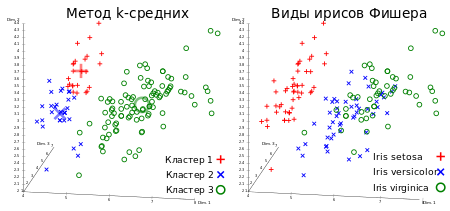
\includegraphics[scale=0.6]{kmeans.png}
	\caption{Результат работы k-means}
	\end{figure}
\end{frame}

\begin{frame}
Достоинства:
	\begin{itemize}
	\item Алгоритм очень гибкий
	\item Простой
	\end{itemize}
Недостатки:
	\begin{itemize}
	\item Кластеризация очень сильно зависит от начального приближения
	\item Кластеризация может быть неадекватной, если изначально было выбрано неверное число кластеров.
	\item Необходимость самостоятельно задавать число кластеров;
	\item Форма кластеров только сферическая. 
	\end{itemize}
\end{frame}

\section[Иерархическая кластеризация]{Иерархическая кластеризация}
\subsection[Агломеративная кластеризация]{Агломеративная кластеризация}

\begin{frame}\frametitle{Алгоритм Ланса-Уильямса}
\begin{enumerate}
	\item Инициализировать множество кластеров $C_1$:
		$t=1; \quad C_t = \{\{x_1\}, \dots \{ x_m\}\}; 
		R(\{x_i\}, \{x_j\})=\rho(x_i, x_j);$
	\item \textbf{Для всех} $t=2, \dots, m$
	\item   \quad найти в $C_{t-1}$ два ближайших кластера: 

		\quad $(U, V) = \arg \min_{U \neq V} R(U, V); R_t=R(U, V);$
	\item   \quad слить их в один кластер: 

		\quad $W=U \cup V; C_t=C_{t-1} \setminus \{U, V\} \cup \{W\};$
	\item   \quad \textbf{для всех} $S \in C_t$
	\item     \qquad вычислить расстояние $R(W,S)$ 

		\qquad по формуле Ланса-Уильямса.
	\end{enumerate}
\end{frame}

\begin{frame}
	\frametitle{Формула Ланса-Уильямса} 
	\begin{multline*}
		R(W, S) = \alpha_U R(U, S) + \alpha_V R(V, S) + \\
		\beta R(U, V) + \gamma | R(U,S) - R(V, S) |,
	\end{multline*}
	где $\alpha_U, \alpha_V, \beta, \gamma$ --- числовые параметры.
\end{frame}

\begin{frame}
\begin{itemize}
	\item Расстояние ближнего соседа:
		$$R^{\text{б}}(W, S) = \min_{w \in W, s \in S} \rho(w, s);$$ $$\alpha_U=\alpha_V=1/2,\enspace \beta=0,\enspace \gamma=-1/2;$$
	\item Расстояние дальнего соседа:
		$$R^{\text{д}}(W, S) = \max_{w \in W, s \in S} \rho(w, s);$$ $$\alpha_U=\alpha_V=1/2,\enspace \beta=0,\enspace \gamma=1/2;$$
	\item Среднее расстояние:
		$$R^{\text{с}}(W, S) = \frac{1}{ |W| |S| } \sum_{w \in W} \sum_{s \in S} \rho(w, s);$$ $$\alpha_U=\frac{|U|}{|W|},\enspace \alpha_V=\frac{|V|}{|W|},\enspace \beta=\gamma=0;$$
\end{itemize}
\end{frame}

\begin{frame}
\begin{itemize}
		
	\item Расстояние между центрами:
		$$\scalebox{0.9}{$R^{\text{ц}}(W, S) = \rho^2 \left( \sum_{w \in W} \frac{w}{|W|}, \sum_{s \in S} \frac{s}{|S|}\right)$};$$ 
		$$\scalebox{0.9}{$\alpha_U=\frac{|U|}{|W|},\enspace \alpha_V=\frac{|V|}{|W|},\enspace \beta= -\alpha_U \alpha_V,\enspace \gamma=0$};$$
	\item Расстояние Уорда:
		$$\scalebox{0.9}{$R^{\text{ц}}(W, S) = \frac{|S| |W|}{|S| + |W|} \rho^2 \left( \sum_{w \in W} \frac{w}{|W|}, \sum_{s \in S} \frac{s}{|S|}\right)$};$$ 
		$$\scalebox{0.9}{$\alpha_U=\frac{|S|+|U|}{|S|+|W|},\enspace \alpha_V=\frac{|S|+|V|}{|S|+|W|},\enspace \beta= -\frac{-|S|}{|S|+|W|},\enspace \gamma=0$};$$

	\item Гибкое расстояние: $$\scalebox{0.9}{$\alpha_U=\alpha_V=\frac{1-\beta}{2},\enspace \beta<1 \;(-0.25),\enspace \gamma=0$};$$
	
	\end{itemize}

\end{frame}

\begin{frame}\frametitle{Свойства кластеризаций}
	\begin{itemize}
	\item Монотонность: кластеризация монотонна, если при каждом объединении расстояния между объединяемыми кластерами только увеличивается.
	\item Кластеризация сжимающая, если $R_t \leq \rho(\mu_U, \mu_V), \forall t$.
	\item Кластеризация растягивающая, если $R_t \geq \rho(\mu_U, \mu_V), \forall t$.
	\end{itemize}
\end{frame}

\begin{frame}
\begin{figure}
	\centering
	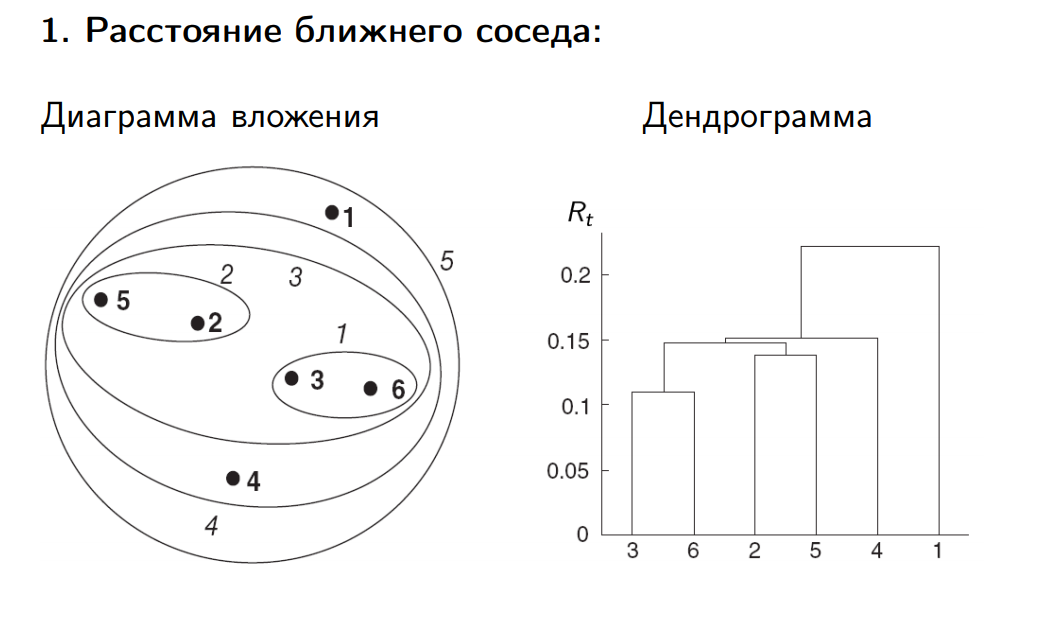
\includegraphics[scale=0.4]{near.png}
\end{figure}
\end{frame}

\begin{frame}
\begin{figure}
	\centering
	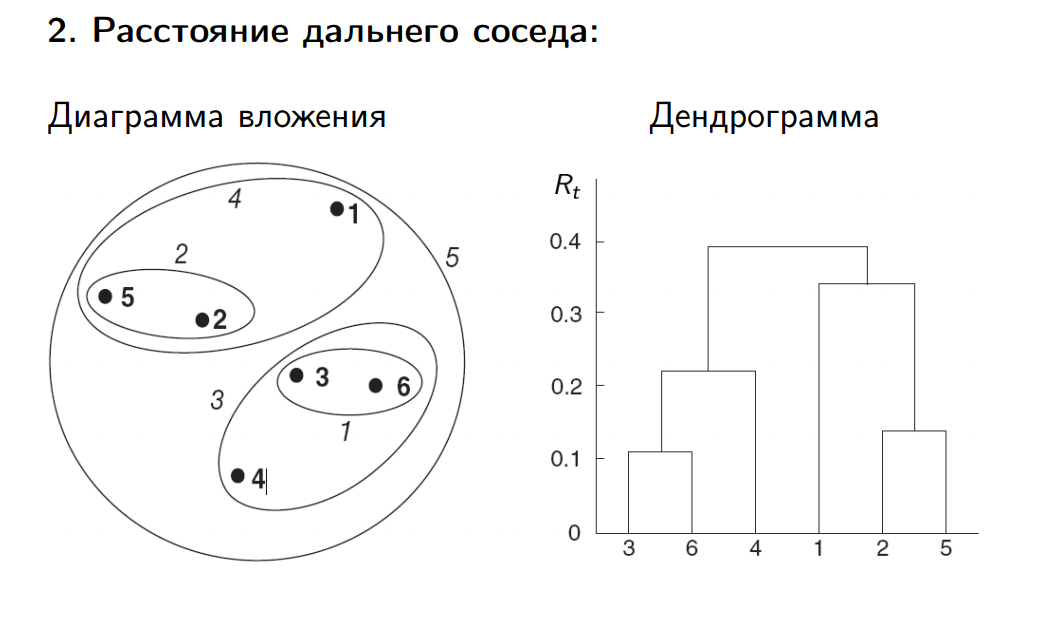
\includegraphics[scale=0.4]{comp.png}
\end{figure}
\end{frame}

\begin{frame}
\begin{figure}
	\centering
	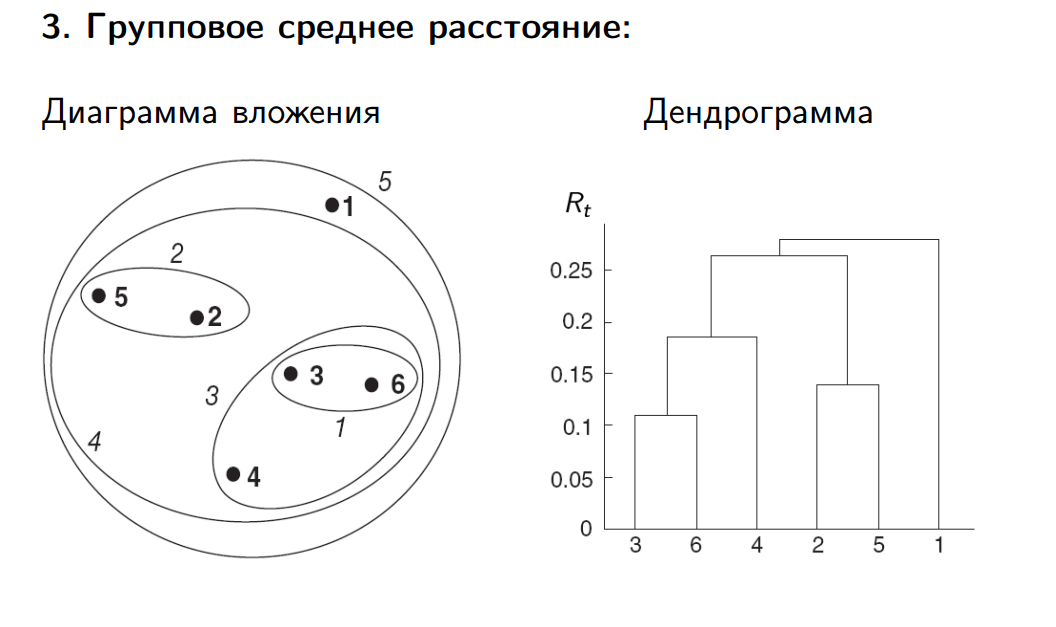
\includegraphics[scale=0.4]{mean.png}
\end{figure}
\end{frame}

\begin{frame}
\begin{figure}
	\centering
	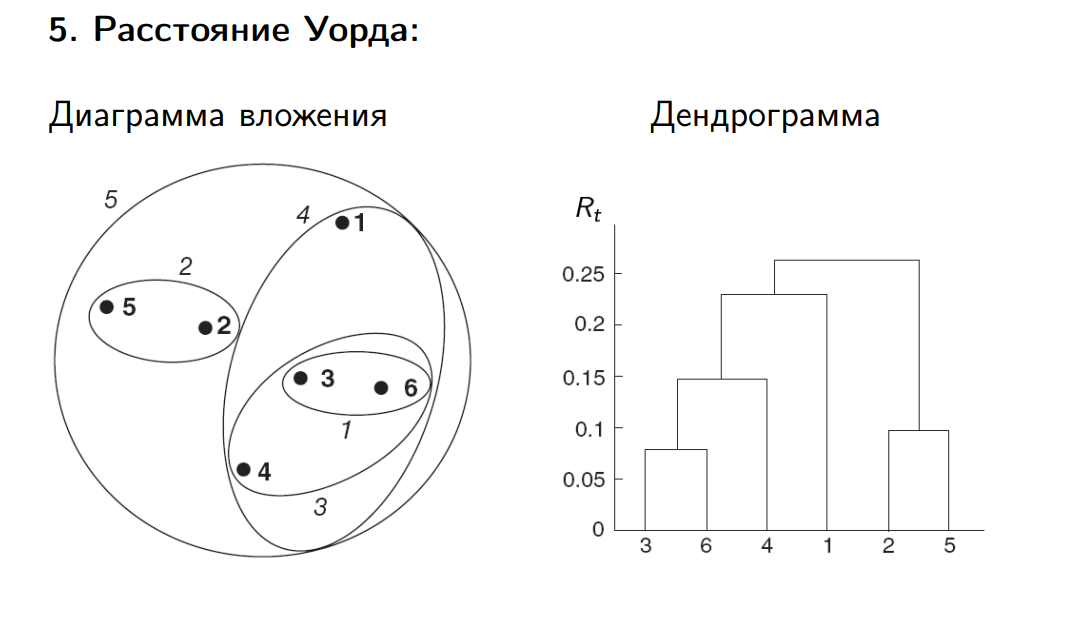
\includegraphics[scale=0.4]{ward.png}
\end{figure}
\end{frame}

\begin{frame}\frametitle{Плюсы и минусы}
Достоинства:
	\begin{itemize}
	\item В качестве результата можно получить дендрограмму.
	\item Форма кластеров может быть произвольной.
	\item Количество кластеров можно определить по дендрограмме.
	\end{itemize}
Недостатки:
	\begin{itemize}
	\item Необходимость подбирать одно из множества различных расстояний.
	\item Отсутствие модели в задаче не позволяет однозначно предпочесть одно разделение на кластеры другому.
	\end{itemize}

\end{frame}

\section[Функционалы качества]{Функционалы качества}

\begin{frame}[shrink=15]\frametitle{Функционалы качества}
Задачу кластеризации можно ставить следующим образом: необходимо приписать номера кластеров
 объектам так, чтобы значение выбранного функционала качества было минимальным или максимальным.
\medskip

Некоторые функционалы качества:
	\begin{itemize}
	\item Среднее внутрикластерное расстояние $F_0=\frac{\sum_{i<j} [y_i=y_j] \rho(x_i, x_j)}{\sum_{i<j} [y_i=y_j]}$
		\medskip

	\item Среднее межкластерное расстояние $F_1=\frac{\sum_{i<j} [y_i \neq y_j] \rho(x_i, x_j)}{\sum_{i<j} [y_i \neq y_j]}$
	\item Силуэт
	\item Индекс Данна и т.д.
	\end{itemize}

	Имеет смысл также вычислять отношение пары функционалов, чтобы учесть как внутрикластерные, так и межкластерные расстояния: $F_0/F_1 \rightarrow min$.
\end{frame}

\begin{frame}\frametitle{Силуэт}
	\begin{enumerate}
		\item Принадлежность объекта своему кластеру $c(x_i) = \frac{1}{|K_i| - 1} \sum_{x_j \in K_i, i \neq j} \rho(x_i, x_j)$

		\item Принадлежность объекта другому кластеру $b(x_i) = \min_{l \neq i} \frac{1}{|K_l|} \sum_{x_j \in K_l} \rho(x_i, x_l)$

		\item Определим силуэт объекта как $s(x_i) = \frac{b(x_i) - c(x_i)}{\max \{ c(x_i), b(x_i) \}}$, если $|K_i| > 1$ и $s(x_i) =0 $, если $|K_i|=1$.

		\item $S = \frac{1}{m} \sum_{i=1}^m s(x_i)$ --- силуэт кластеризации.
	\end{enumerate}
\end{frame}

\begin{frame}\frametitle{Dunn index}
	$$D = \frac{\min_{1 \leq i < j < k} \delta(K_i, K_j)}{\max_{1 \leq s \leq k} \Delta(K_s)},$$
	где $\delta(K_i, K_j)$ --- расстояние между кластерами, $\Delta(K_s)$ --- диаметр кластера.
\end{frame}

\begin{frame}
	Если доступна внешняя информация о разделении на классы априори, то можно воспользоваться следующими метриками:
	\begin{itemize}
		\item Rand Index $$\scalebox{0.9}{$Rand = \frac{TP + FN}{TP + TN +FP +FN}$}$$
	\item Jaccard Index $$\scalebox{0.9}{$Jaccard = \frac{TP}{TP+TN+FP}$}$$
	\item Minkowski Score
	\item Folkes and Mallows Index и т.д.
	\end{itemize}
	\end{frame}


\section[Другие эвристические алгоритмы]{Другие эвристические алгоритмы}

\subsection[FOREL]{FOREL}

\begin{frame} \frametitle{Кратчайший незамкнутый путь (КНП)}
	\begin{enumerate}
	\item Найти пару вершин $(x_i, x_j) \in X^m$ с наименьшим $\rho(x_i, x_j)$ и соединить их ребром;
	\item \textbf{Пока} в выборке остаются изолированные точки
	\item \quad найти изолированную точку, ближайшую к 

		\quad некоторой неизолированной;
	\item \quad соединить эти две точки ребром;
	\item удалить $k-1$ самых длинных рёбер;
	\end{enumerate}
\end{frame}

\begin{frame}[shrink=20] \frametitle{FOREL}
	\begin{enumerate}
	\item Пусть $U=X^m$
	\item \textbf{Пока} есть некластеризованные точки, т.е. $U \neq \varnothing$;
	\item \quad взять случайную точку $x_0 \in U$;
	\item \quad \textbf{Повторять}
	\item \qquad образовать кластер с центром в $x_0$ и радиусом $R$:

		\qquad $K_0 = \{ x_i \in U ~|~ \rho(x_i, x_0) \leq R \};$
	\item \qquad переместить центр $x_0$ в центр масс кластера:

		\qquad $x_0 = \frac{1}{|K_0|} \sum_{x_i \in K_0} x_i;$
	\item \quad \textbf{Пока} состав кластера $K_0$ не стабилизируется;
	\item \quad $U= U \setminus K_0;$
	\item применить алгоритм КНП к множеству центров кластеров;
	\item каждый $x_i \in X^m$ приписать кластеру с ближайшим центром;
	\end{enumerate}
\end{frame}

\begin{frame}\frametitle{Плюсы и минусы}
	Достоинства:
	\begin{itemize}
		\item Получаем двухуровневую систему кластеров;
		\item Кластеры могут быть произвольной формы;
		\item варьируя $R$ можно управлять детальностью кластеризации.
	\end{itemize}
	Недостатки:
	\begin{itemize}
		\item алгоритм очень чувствителен к $R$ и к начальному выбору точки $x_0$
	\end{itemize}
\end{frame}

\subsection[DBSCAN]{DBSCAN}

\begin{frame}\frametitle{Density-Based Spatial Clustering of Aplications with Noise (DBSCAN)}
	Объект $x \in U$, его $\eps$-окрестность $U_\eps (x) = \{u \in U : \rho(x ,u ) \leq \eps\}$
	Каждый объект может быть одного из трёх типов:
	\begin{itemize}
	\item корневой: имеет плотную окрестность $|U_\eps (x)| \geq m$
	\item граничный: не корневой, но находится в окрестности корневого
	\item выброс: не корневой и не граничный.
	\end{itemize}
\end{frame}

\begin{frame}
	\begin{enumerate}
		\item $U=X^m$, $N=\varnothing$, $z=0$;
		\item \textbf{Пока} есть некластеризованные точки, т.е. $U \neq \varnothing$;
		\item \quad взять случайную точку $x \in U$;
		\item \quad \textbf{если} $|U_\eps (x)| < m$, \textbf{то}
		\item \qquad пометить $x$ как шумовой;
		\item \quad \textbf{иначе}
		\item  \qquad создать новый кластер: $K=U_\eps (x)$; $z = z + 1$;
		\item \qquad \textbf{для всех} $x' \in K$
		\item \hskip 3em \textbf{если} $|U_\eps (x')| \geq m$ \textbf{то} $K=K \cup U_\eps(x')$;
		\item \hskip 3em \textbf{иначе} пометить $x'$ как граничный элемент $K$;
		\item \qquad $a(x_i) = z$ для всех $x' \in K$;
		\item \qquad $U=U \setminus K$;
	\end{enumerate}
\end{frame}

\begin{frame}
	\begin{figure}
	\centering
	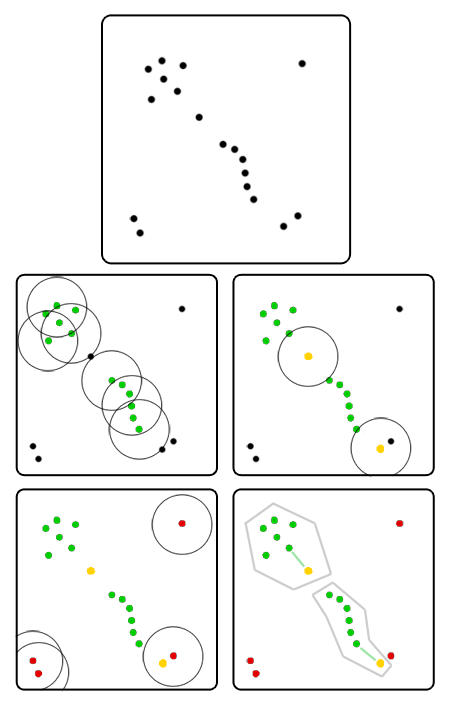
\includegraphics{dbscan.png}
	\caption{Иллюстрация к алгоритму DBSCAN}
	\end{figure}
\end{frame}

\begin{frame}
	\begin{figure}
	\centering
		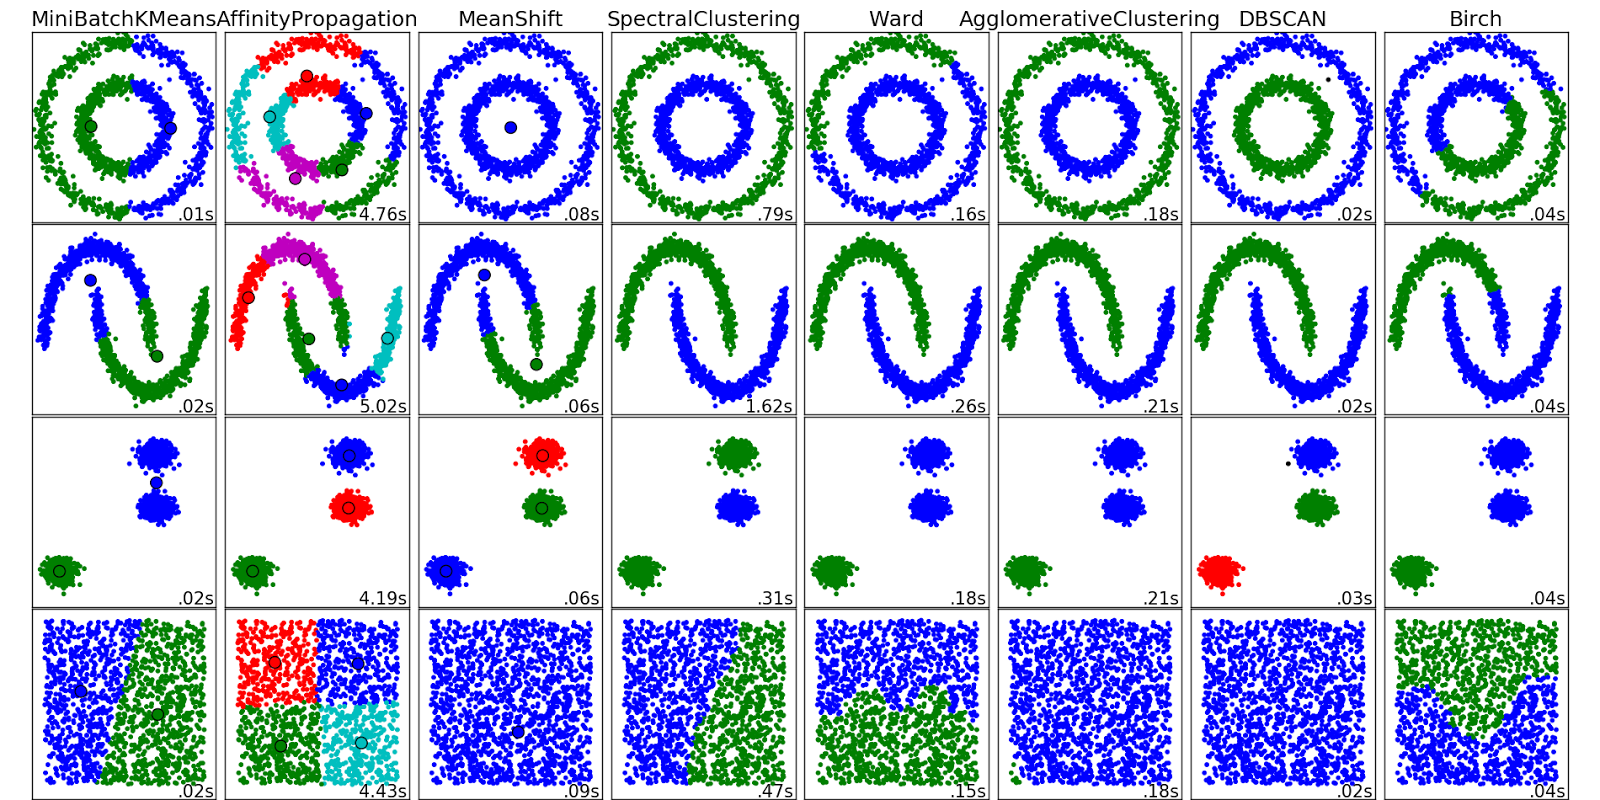
\includegraphics[scale=0.2]{dbscanexamp.png}
		\caption{Пример работы DBSCAN (второй столбец справа)}
	\end{figure}
\end{frame}


\begin{frame}\frametitle{Плюсы и минусы}
	Достоинства:
	\begin{itemize}
		\item Быстрая кластеризация больших данных (от $O(m \ln m)$ до $O(m^2)$ в зависимости от реализации);
		\item Кластеры произвольной формы;
		\item Явная разметка шумовых объектов;
		\item Хорошо поддаётся модифицированию (существуют реализации, скрещенные с k-means и даже с GMM).
	\end{itemize}
	Недостатки:
	\begin{itemize}
	\item Алгоритм может неадекватно обрабатывать сильные вариации плотности данных внутри кластера, проёмы и шумовые мосты между кластерами.
	\end{itemize}
\end{frame}

\end{document}
